\documentclass[tikz,border=5]{standalone}
\usetikzlibrary{matrix,arrows.meta}
\usepackage{tikz-cd}
\usetikzlibrary{arrows,calc}
\usepackage{xypic}
\begin{document}


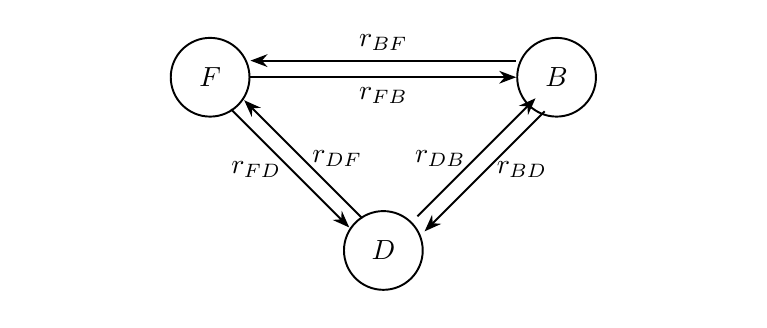
\begin{tikzpicture}[>=Stealth,->,line width=.7pt]
\matrix [matrix of math nodes,
column sep={2.2cm,between origins},
row sep={2.2cm,between origins},
nodes={circle, draw, minimum size=1cm}]
{
& |(1)| F &   & |(2)| B & \\
&  & |(3)| D & \\};

\draw (1)--(2) node [midway, below] {$r_{FB}$}; 
\draw[transform canvas={xshift=0pt,yshift=6pt}] (2)--(1) node [midway, above] {$r_{BF}$};



\draw[transform canvas={xshift=2pt,yshift=2pt},shorten <= -1pt]  (3)-- (1)  node[midway, right] {$r_{DF}$};
\draw[transform canvas={xshift=-2pt,yshift=-2pt},shorten <= -1pt] (1)--(3)
node[midway, left] {$r_{FD}$};

\draw[transform canvas={xshift=2pt,yshift=2pt},shorten >= -1pt] (3)--(2) node[midway, left] {$r_{DB}$};;
\draw[transform canvas={xshift=6pt,yshift=-2pt},shorten >= -2pt] (2)--(3) node[midway, right] {$r_{BD}$};

\end{tikzpicture}
\end{document}
